\section{实验三\ \ 进程管理}

\subsection{实验目的}
\begin{enumerate}
    \item 了解和掌握操作系统中进程创建的实现原理。
    \item 了解和掌握操作系统中进程主动释放CPU资源(yield)的流程方法。
    \item 了解和掌握操作系统中进程循环轮转调度的实现原理。
    \item 了解和掌握操作系统中进程等待机制的实现原理。
    \item 了解和掌握操作系统中信号量的原理及实现。
\end{enumerate}

\subsection{实验内容}
\paragraph{lab3_1 进程创建} 本实验需要在PKE操作系统内核中实现子进程到父进程代码段的映射,以最终完成fork动作。由于实验涉及的父进程只包含代码段,而不包含数据段内容,因此只需要将父进程代码段映射到子进程对应虚地址处即可。

从测试程序使用的fork函数出发,执行类似lab1_1的系统调用路径跟踪,发现kernel/syscall.c中的sys_user_fork系统调用函数调用了kernel/process.c中的do_fork函数,该函数已部分完成,其中代码段映射部分缺失,因此实验只需要补充代码段的映射代码即可。代码段的映射首先需要获得父进程代码段的虚地址va及其映射的物理地址pa,然后按照合适的权限(可读可执行)在子进程页表中登记该映射关系,并在子进程mapped_info结构中登记该页面相关信息即可。函数补充的代码如下,函数中部分已实现的代码使用“......”省略代替。
\begin{cppcode}
int do_fork( process* parent ) {
  ......
  for( int i=0; i<parent->total_mapped_region; i++ ){
    uint64 pa, va, perm;
    switch( parent->mapped_info[i].seg_type ){
      ......
      case CODE_SEGMENT:
        pa = lookup_pa(parent->pagetable, parent->mapped_info[i].va);
        va = parent->mapped_info[i].va;
        perm = prot_to_type(PROT_EXEC | PROT_READ, 1);
        sprint("do_fork map code segment at pa:%lx of parent to child at va:%lx.\n", pa, va);
        map_pages(child->pagetable, va, PGSIZE, pa, perm); 
        
        child->mapped_info[child->total_mapped_region].va = parent->mapped_info[i].va;
        child->mapped_info[child->total_mapped_region].npages = 
        parent->mapped_info[i].npages;
        child->mapped_info[child->total_mapped_region].seg_type = CODE_SEGMENT;
        child->total_mapped_region++;
        break;
    }
  }
  ......
  return child->pid;
}
\end{cppcode}
\paragraph{lab3_2 进程yield}
进程主动释放CPU资源使用了yield系统调用实现,跟踪系统调用路径,发现该系统调用使用了kernel/syscall.c中的sys_user_yield系统调用函数,该函数尚未实现。进程释放CPU的步骤为:
\begin{enumerate}
    \item 将当前进程加入到就绪队列的队尾,并置为就绪(READY)状态
    \item 转进程调度
\end{enumerate}
由于进程相关操作函数已在sche.c中实现,因此只需要首先调用insert_to_ready_queue函数,将当前进程加入到就绪队列的队尾(该函数同时会将当前进程设置为就绪状态),然后调用schedule函数转进程调度。sys_user_yield函数代码实现如下,其中current是指向当前进程结构(process)的指针。

\begin{cppcode}
ssize_t sys_user_yield() {
  insert_to_ready_queue(current);
  schedule();
  return 0;
}
\end{cppcode}
\paragraph{lab3_3 循环轮转调度} 
类似lab3_2,循环轮转调度测试程序仍会产生父、子两个进程,并执行大循环操作,不同于lab3_2,本实验的父子进程均不会主动释放CPU资源。为避免一个进程占用过长的CPU时间,需要操作系统基于时间片分片的原理执行进程轮转调度。在lab1_3中,我们已经实现了时钟中断的基本响应,因此可以基于时钟中断实现进程的轮转调度。

基于时间片的进程轮转调度首先需要定义时间片长度,该长度在kernel/sched.h文件中定义:
\begin{cppcode}
//length of a time slice, in number of ticks
#define TIME_SLICE_LEN  2
\end{cppcode}
时间片长度定义为 $2$,即每经过 $2$ 个tick执行一次进程轮转调度。

在kernel/strap.c文件中,CAUSE_MTIMER_S_TRAP类型的trap用于处理时钟中断,除了lab1_3实现的handle_mtimer_trap函数外,本实验增加了rrsched函数用于实现进程循环轮转调度,即每次时钟中断来临时,除了处理时钟中断之外,还需要检查当前进程发生时钟中断次数current->tick_count是否达到定义的时间片长度TIME_SLICE_LEN,若达到该长度,则将current->tick_count清零,并将当前进程插入就绪队列尾部,之后转进程调度;否则将current->tick_count计数器加一。rrsched函数的实现如下。
\begin{cppcode}
void rrsched() {
    if (current->tick_count + 1 >= TIME_SLICE_LEN) {
        current->tick_count = 0;
        insert_to_ready_queue(current);
        schedule();
    }
    else {
        current->tick_count++;
    }
}
\end{cppcode}

\paragraph{lab3_challenge1 进程等待和数据段复制} 
进程等待,即wait系统调用,在操作系统中具有非常重要的地位,它不仅可以释放僵尸进程的资源,还可以实现进程同步。实验中需要实现的wait函数wait函数接受一个参数“pid”,参数取值及功能定义如下:
\begin{enumerate}
    \item pid = -1:父进程等待任意一个子进程结束即返回子进程的pid。
    \item pid > 0:父进程等待进程号为pid的子进程退出即返回子进程的pid。
    \item pid > 0 但不是父进程的子进程或pid取其他非法值:返回-1。
\end{enumerate}
为实现wait函数,首先需要在kernel/syscall.h中注册wait系统调用号,如下。
\begin{cppcode}
#define SYS_user_wait (SYS_user_base + 6)
\end{cppcode}
根据系统调用路径,需要在kernel/syscall.c的do_syscall函数中增加以下case语句。
\begin{cppcode}
case SYS_user_wait:
    return sys_user_wait(a1);
\end{cppcode}
同时还需要实现sys_user_wait函数,函数的框架如下。

\begin{cppcode}
ssize_t sys_user_wait(int pid) {
    if (pid == -1) {
        ......
    } else if (pid > 0) {
        ......
    } else return -1;
}
\end{cppcode}
即分三种情况对pid不同取值的情况进行处理。

在具体实现wait系统调用函数sys_user_wait之前,首先需要实现等待队列和进程资源释放函数。

等待队列的实现需要在已有代码的基础上补充必要的数据结构以及等待队列相关操作函数。

在数据结构方面,考虑到wait系统调用具有多种等待原因(如等待某一个特定子进程或任意子进程结束),故需要增加waiting_for变量记录当前进程的等待目标。由于等待队列未必是先进先出的,后进的进程可能因为其等待目标的结束而提前被调度运行,因此等待队列应该是双链表。故kernel/process.h中定义的process结构中需要增加以下字段。
\begin{cppcode}
typedef struct process {
    ......
    // next queue element
    struct process *queue_next;
    // prev queue element
    struct process *queue_prev;
    // blocking reason
    int waiting_for;        // -1: any son, positive integer: a certain son
    ......
}
\end{cppcode}
同时还需要在kernel/process.c中定义等待队列头部指针,如下。
\begin{cppcode}
// waiting queue
process* waiting_queue_head = NULL;
\end{cppcode}

在完成了等待队列数据结构定义后,还需要定义等待队列相关操作函数。等待队列插入函数首先需要判断当前等待队列是否为空,若为空则将当前进程作为等待队列头部;若等待队列非空,则首先遍历队列确保当前进程不在等待队列中,然后将当前进程插入等待队列末尾,设置等待原因、置当前进程的状态为BLOCKED。等待队列插入函数在kernel/process.c中定义如下。
\begin{cppcode}
void insert_to_waiting_queue( process* proc, int waiting_for ) {
    if (waiting_queue_head == NULL) {
        proc->status = BLOCKED;
        proc->queue_next = NULL;
        proc->queue_prev = NULL;
        proc->waiting_for = waiting_for;
        waiting_queue_head = proc;
        return;
    }
    
    process *p;
    for (p = waiting_queue_head; p->queue_next != NULL; p = p->queue_next)
        if (p == proc) return;  // Already in queue
        
    if (p == proc) return;      // Test the last element
    p->queue_next = proc;
    proc->queue_prev = p;
    proc->queue_next = NULL;
    proc->status = BLOCKED;
    proc->waiting_for = waiting_for;
    return;
}
\end{cppcode}

除等待队列插入函数外,还需要实现等待队列检查函数。等待队列检查函数传入的参数是指向一个即将结束的进程的指针,该函数遍历等待队列,并与当前函数的信息进行比较,判断等待队列中是否存在可以被唤醒的进程,若存在,则调用insert_to_ready_queue方法将该进程插入就绪队列,同时将该进程从等待队列中删除。等待队列检查函数的实现如下。
\begin{cppcode}
void check_waiting_queue( process* proc ) {
    process *p;
    for (p = waiting_queue_head; p != NULL; p = p->queue_next) {
        if (p == proc->parent && (p->waiting_for == -1 || p->waiting_for == proc->pid)) {
            if (p->queue_prev == NULL) {
                waiting_queue_head = p->queue_next;
                if (p->queue_next != NULL) p->queue_next->queue_prev = NULL;
            } else if (p->queue_next == NULL) {
                p->queue_prev->queue_next = NULL;
            } else {
                p->queue_next->queue_prev = p->queue_prev;
                p->queue_prev->queue_next = p->queue_next;
            }
            insert_to_ready_queue(p);
        }
    }
    return;
}
\end{cppcode}

至此,等待队列部分已全部实现。

由于进程的结束仅仅将其状态标记为ZOMBIE,并没有真正释放资源,故还需要实现进程资源释放函数distruct_space,用以实现进程资源的释放,该函数实现如下。
\begin{cppcode}
int distruct_space( process* proc ) {
    for (int i = 0; i < proc->total_mapped_region; i++) {
        for (int j = 0; j < proc->mapped_info[i].npages; j++) {
            if (proc->mapped_info[i].seg_type != CODE_SEGMENT)
                free_page((void *)lookup_pa(proc->pagetable, proc->mapped_info[i].va + j * PGSIZE));
        }
    }
    free_page((void *)proc->mapped_info);
    free_page((void *)(proc->kstack - PGSIZE));
    free_page((void *)proc->pagetable);
    free_page((void *)proc->trapframe);

    return 0;
}
\end{cppcode}

下文基于实现的等待队列及进程资源释放函数具体实现wait系统调用函数sys_user_wait。

对于pid = -1的情况,需要首先遍历所有进程,查看是否有已经结束的子进程,若有则直接调用distruct_space函数释放该进程资源,并返回该子进程的pid;若不存在已结束的子进程,则将当前进程插入等待队列,等待原因为“-1”,转进程调度,直到某个子进程结束将其唤醒,方可继续执行,释放该子进程资源,并返回该子进程的pid。此部分代码实现如下。
\begin{cppcode}
    if (pid == -1) {
        int i;
        int flag = 0;                   // flag of weather pid is valid
        for (i = 0; i < NPROC; i++) {   // find a current exited ZOMBIE son
            if (procs[i].parent == current) {
                flag = 1;                           // -1 is legal, which means parent is a son
                if (procs[i].status == ZOMBIE) {    // the son is already existed
                    distruct_space(&procs[i]);
                    procs[i].status = FREE;
                    return procs[i].pid;
                }
            }
        }
        if (!flag) return -1;   // pid does not have a son
        while(1){               // make sure that the parent awaken properly
            insert_to_waiting_queue(current, -1);   // none of the sons exited
            schedule();
            for (i = 0; i < NPROC; i++) {           // find the ZOMBIE son return from
                if (procs[i].parent == current && procs[i].status == ZOMBIE) {
                    distruct_space(&procs[i]);
                    procs[i].status = FREE;
                    return procs[i].pid;
                }
            }
        }
    }
\end{cppcode}

对于pid大于0的情况,需要首先遍历所有进程,判断是否存在进程号为该pid的进程是当前进程的子进程,若不存在,则返回-1;若存在,则判断该进程是否为ZOMBIE状态,若不是则将当前进程插入等待队列,等待原因为pid,转进程调度。后续处理和上文相仿,不再赘述。此部分代码实现如下。
\begin{cppcode}
    else if (pid > 0) {
        int i;
        for (i = 0; i < NPROC; i++) {
            if (procs[i].pid == pid) {
                if (procs[i].parent != current) {
                    return -1;  // pid illegal
                }
                while(1) {
                    if (procs[i].status != ZOMBIE) {
                        insert_to_waiting_queue(current, pid);
                        schedule();
                    }
                    distruct_space(&procs[i]);
                    procs[i].status = FREE;
                    return procs[i].pid;
                }
            }
        }
        return -1;      // pid illegal
    }
}
\end{cppcode}

对于pid取值为其他的情况,为非法情况,直接返回-1即可。

此外,由于实验的测试程序使用了全局变量,因此还需要在lab3_1实现的简单进程创建功能的基础上增加数据段的复制功能,以保证父子进程之间数据段相互独立。数据段的复制功能需要在kernel/process.c文件中的do_fork函数内增加case DATA_SEGMENT的内容,首先根据父进程页表和数据段虚拟地址获得父进程数据段的物理地址,然后使用alloc_page方法申请一页物理页面,再使用memcpy函数执行物理页面内容的拷贝,最后使用map_pages方法执行虚实地址间的映射。数据段的赋值部分代码如下。
\begin{cppcode}
    case DATA_SEGMENT:
        pa = lookup_pa(parent->pagetable, parent->mapped_info[i].va);
        child_pa = (uint64)alloc_page();
        memcpy( (void *)child_pa, (void *)pa, PGSIZE );
        va = parent->mapped_info[i].va;
        perm = prot_to_type(PROT_WRITE | PROT_READ, 1);
        map_pages(child->pagetable, va, PGSIZE, child_pa, perm);

        child->mapped_info[child->total_mapped_region].va = parent->mapped_info[i].va;
        child->mapped_info[child->total_mapped_region].npages =
                parent->mapped_info[i].npages;
        child->mapped_info[child->total_mapped_region].seg_type = DATA_SEGMENT;
        child->total_mapped_region++;
        break;
\end{cppcode}

至此,进程等待和数据段赋值功能已经全部实现。
\paragraph{lab3_challenge2 实现信号量} 
信号量是操作系统中另一重要工具,它在进程同步中起着至关重要的作用。信号量的实现首先需要在kernel/syscall.h中定义信号量结构SEM和信号量状态sem_status,以及最大支持的信号量数目,定义如下。其中SEM的status取值为S_FREE或S_USING。
\begin{cppcode}
enum sem_status {
    S_FREE,               // unused state
    S_USING,              // using state
};

typedef struct SEM {
    int value;
    int status;
    process* waiting_queue_head;    // pointer of the head of waiting queue
}SEM;

#define MAX_SEM 64
\end{cppcode}

完成信号量结构定义之后,需要在kernel/syscall.c中定义信号量数组和记录当前已申请信号量数目的变量,如下。
\begin{cppcode}
SEM sem[MAX_SEM];
int used_sem = 0;
\end{cppcode}

信号量有关系统调用共有三个,分别是:sem_new(创建信号量)、sem_P(信号量的P操作)和sem_V(信号量的V操作)。为实现这三个系统调用,需要首先在kernel/syscall.h中注册相应系统调用号,如下。
\begin{cppcode}
#define SYS_user_sem_new (SYS_user_base + 6)
#define SYS_user_sem_V (SYS_user_base + 7)
#define SYS_user_sem_P (SYS_user_base + 8)
\end{cppcode}
之后需要在kernel/syscall.c中do_syscall函数内增加三个函数的case选择语句,并创建三个函数的函数定义,下文对这三个函数的实现逐一分析。

信号量的创建是使用信号量的第一步,课程设计中使用一次创建一个信号量的实现方式。信号量创建函数sys_user_sem_new接受一个表示创建的信号量初始值的变量v,在信号量尚未用完且v取值合法的情况下,遍历信号量数组,找到第一个信号量状态为S_FREE的信号量作为本次创建的信号量,执行相应的赋值操作并返回该信号量的id。信号量创建的系统调用函数实现如下。
\begin{cppcode}
ssize_t sys_user_sem_new(int v) {
    if (used_sem >= MAX_SEM || v < 0) return -1;
    for (int i = 0; i < MAX_SEM; i++) {
        if (sem[i].status == S_FREE) {
            sem[i].status = S_USING;
            sem[i].value = v;
            used_sem++;
            return i;
        }
    }
    return -1;
}
\end{cppcode}

信号量的V操作即释放一个资源,需要将给定id的信号量值增加1,并判断增加后的信号量值是否大于0,若是则直接返回,否则还需要进一步检查该信号量对应的等待队列是否为空,若不为空则将等待队列首部进程弹出,并加入就绪队列,表示该进程可以获得一个正在等待的此类资源,因而可以被唤醒。V操作的具体实现如下。
\begin{cppcode}
ssize_t sys_user_sem_V(int sem_id) {
    if (sem[sem_id].status == S_FREE) return -1;
    if (++sem[sem_id].value > 0) return 0;
    else if (sem[sem_id].waiting_queue_head == NULL) return 0;
    else {
        insert_to_ready_queue(sem[sem_id].waiting_queue_head);
        sem[sem_id].waiting_queue_head = sem[sem_id].waiting_queue_head->queue_next;
    }
    return 0;
}
\end{cppcode}

信号量的P操作即请求一个资源,需要将给定id的信号量值减一,并判断减少后的信号量值是否仍不小于0,若是则直接返回,否则表示该类资源目前不足,需要等待,因此需要将当前进程插入该信号量的等待队列中,之后转进程调度。P操作的具体实现如下。
\begin{cppcode}
ssize_t sys_user_sem_P(int sem_id) {
    if (sem_id >= used_sem || sem[sem_id].status == S_FREE) return -1;
    if (--sem[sem_id].value >= 0) return 0;
    else {
        insert_to_waiting_queue(&sem[sem_id].waiting_queue_head, current);
        schedule();
    }
    return 0;
}
\end{cppcode}

至此,课程设计涉及的信号量相关功能已全部实现。
\subsection{实验调试与测试结果}
\paragraph{lab3_1 进程创建} 进程创建实验的测试程序如下所示,父进程使用fork系统调用创建子进程,父子进程分别打出对应字符串并返回。
%图\ref{fig:lab1-1-testbench}
\begin{cppcode}
#include "user/user_lib.h"
#include "util/types.h"

int main(void) {
  uint64 pid = fork();
  if (pid == 0) {
    printu("Child: Hello world!\n");
  } else {
    printu("Parent: Hello world! child id %ld\n", pid);
  }
  exit(0);
}
\end{cppcode}

编译运行测试程序,程序测试结果如图\ref{fig:lab3-1-testres}所示,程序首先打印了“do_fork map code segment at pa:0000000087fb2000 of parent to child at va:0000000000010000.”,说明子进程到父进程的代码段映射成功完成;之后程序打印了"Parent: Hello world! child id 1"和"Child: Hello world!"两行字符串,并正常退出,说明进程创建实验成功完成。
\begin{figure}[!htbp]
    \centering
    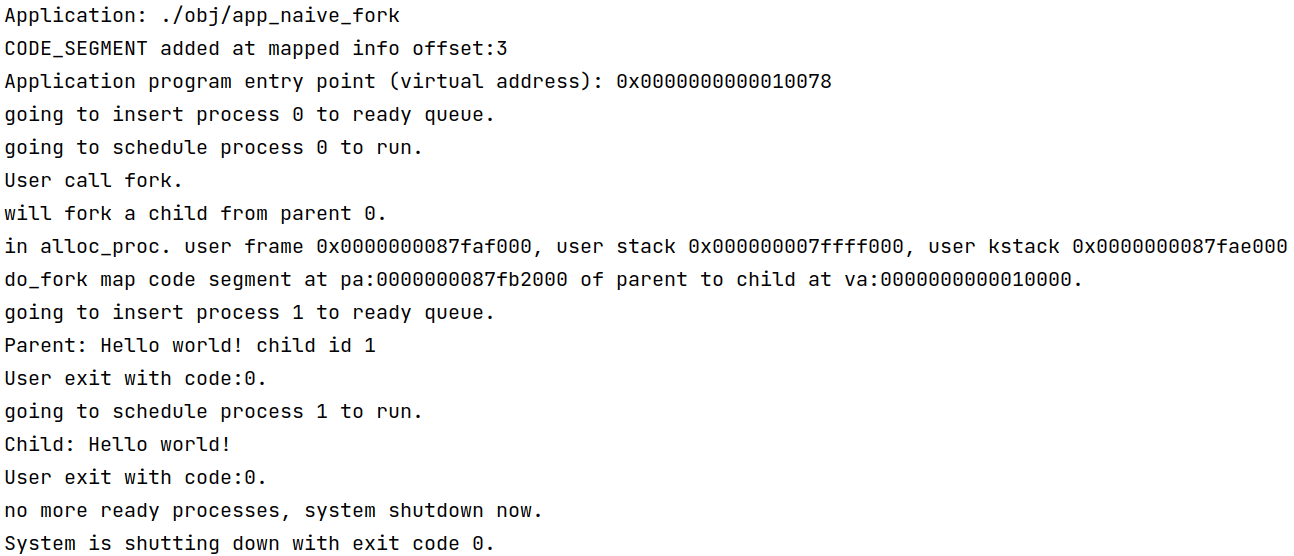
\includegraphics[width = 13cm]{figure/lab3_1_testresult.png}
    \caption{lab3_1进程创建测试结果}
    \label{fig:lab3-1-testres}
\end{figure}

\paragraph{lab3_2 进程yield}
进程yield实验的测试程序如下所示,父子进程分别执行循环次数为rounds的大循环,且每执行10000次调用yield释放CPU资源。由于篇幅限制,循环总数rounds设置为20001。
\begin{cppcode}
#include "user/user_lib.h"
#include "util/types.h"

int main(void) {
  uint64 pid = fork();
  uint64 rounds = 20001;
  if (pid == 0) {
    printu("Child: Hello world! \n");
    for (uint64 i = 0; i < rounds; ++i) {
      if (i % 10000 == 0) {
        printu("Child running %ld \n", i);
        yield();
      }
    }
  } else {
    printu("Parent: Hello world! \n");
    for (uint64 i = 0; i < rounds; ++i) {
      if (i % 10000 == 0) {
        printu("Parent running %ld \n", i);
        yield();
      }
    }
  }
  exit(0);
  return 0;
}
\end{cppcode}

编译运行测试程序,程序测试结果如图\ref{fig:lab3-2-testres}所示。父进程和子进程轮流打印运行次数,并在程序结束后正常退出,说明进程yield实验成功完成。
\begin{figure}[!htbp]
    \centering
    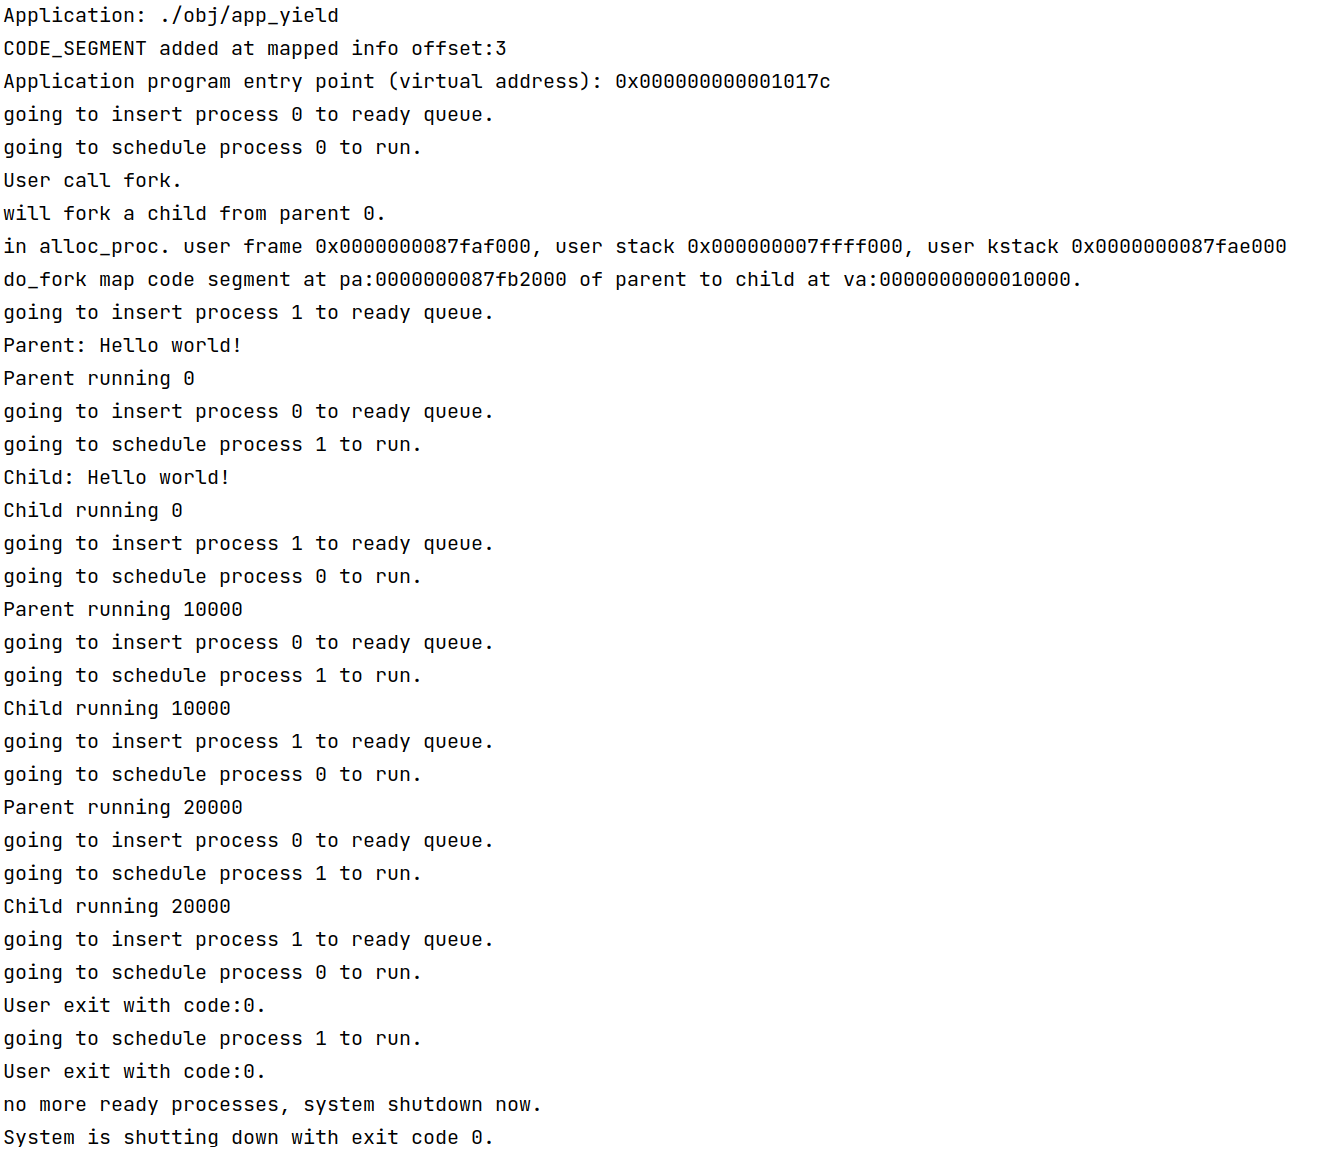
\includegraphics[width = 12cm]{figure/lab3_2_testresult.png}
    \caption{lab3_2进程yield测试结果}
    \label{fig:lab3-2-testres}
\end{figure}
\paragraph{lab3_3  循环轮转调度}
循环轮转调度实验的测试程序如下所示,父子进程分别执行循环次数为rounds的大循环,且每执行10000000次打印当前进程标志及循环次数。由于篇幅限制,循环总数rounds设置为30000001。

\begin{cppcode}
#include "user/user_lib.h"
#include "util/types.h"

int main(void) {
  uint64 pid = fork();
  uint64 rounds = 30000001;
  uint64 interval = 10000000;
  uint64 a = 0;
  if (pid == 0) {
    printu("Child: Hello world! \n");
    for (uint64 i = 0; i < rounds; ++i) {
      if (i % interval == 0) printu("Child running %ld \n", i);
    }
  } else {
    printu("Parent: Hello world! \n");
    for (uint64 i = 0; i < rounds; ++i) {
      if (i % interval == 0) printu("Parent running %ld \n", i);
    }
  }
  exit(0);
  return 0;
}
\end{cppcode}

编译运行测试程序,程序测试结果如图\ref{fig:lab3-3-testres}所示,程序执行过程中每间隔2次tick进行一次进程循环轮转调度,最后一轮执行由于父子进程的执行时间均不到1个tick,故打印结果后正常退出。测试结果表明循环轮转调度实验成功完成。
\begin{figure}[!htbp]
    \centering
    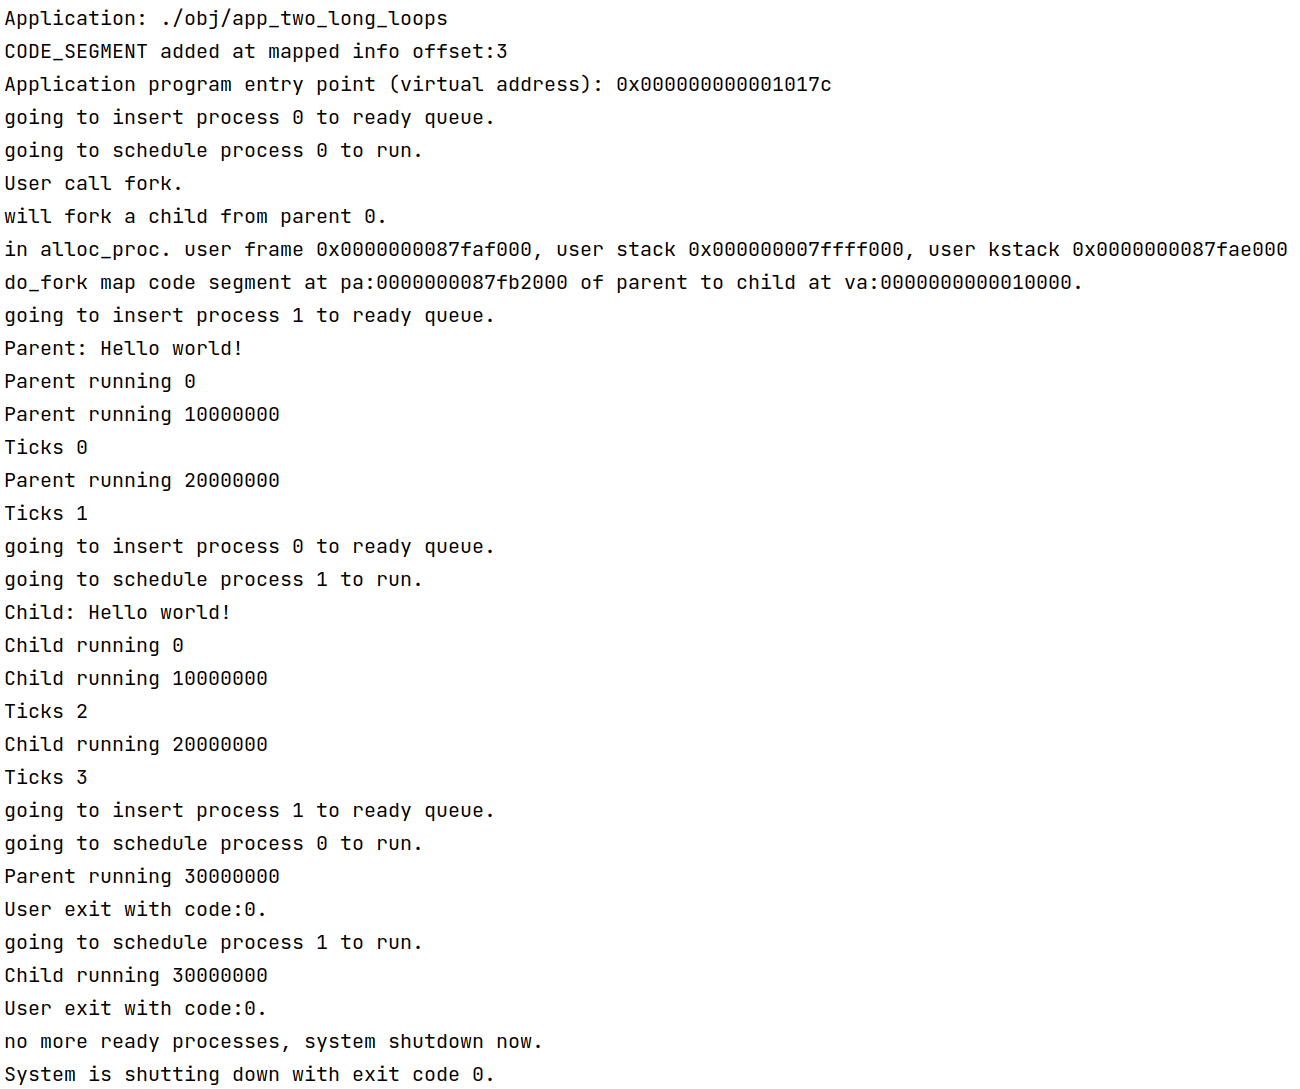
\includegraphics[width = 12cm]{figure/lab3_3_testresult.png}
    \caption{lab3_3循环轮转调度测试结果}
    \label{fig:lab3-3-testres}
\end{figure}

\paragraph{lab3_challenge1 进程等待和数据段复制}
进程等待和数据段复制实验的测试程序如下。该程序依次生成父、子、孙子进程,三个进程分别给自己的全局变量flag赋值为100、10、1,然后等待自己的子进程退出(若存在子进程),最后打印进程标志和flag值并退出。测试程序代码如下。
\begin{cppcode}
#include "user/user_lib.h"
#include "util/types.h"

int flag;
int main(void) {
    flag = 100;
    int pid = fork();
    if (pid == 0) {
        flag = 10;
        pid = fork();
        if (pid == 0) {
            flag = 1;
            printu("Grandchild process end, flag = %d.\n", flag);
        } else {
            wait(pid);
            printu("Child process end, flag = %d.\n", flag);
        }
    } else {
        wait(-1);
        printu("Parent process end, flag = %d.\n", flag);
    }
    exit(0);
    return 0;
}
\end{cppcode}

编译运行测试程序,程序测试结果如图\ref{fig:lab3-c1}所示。进程0执行fork生成进程1,进程1执行fork生成进程2,进程0和1分别等待各自的子进程退出。进程2首先打印自己的flag值(1)并退出,随后进程1被唤醒,打印自己的flag值并退出,最后进程0被唤醒,打印自己的flag值并退出。程序运行结果符合预期,进程等待和数据段复制实验成功完成。
\begin{figure}[!htbp]
    \centering
    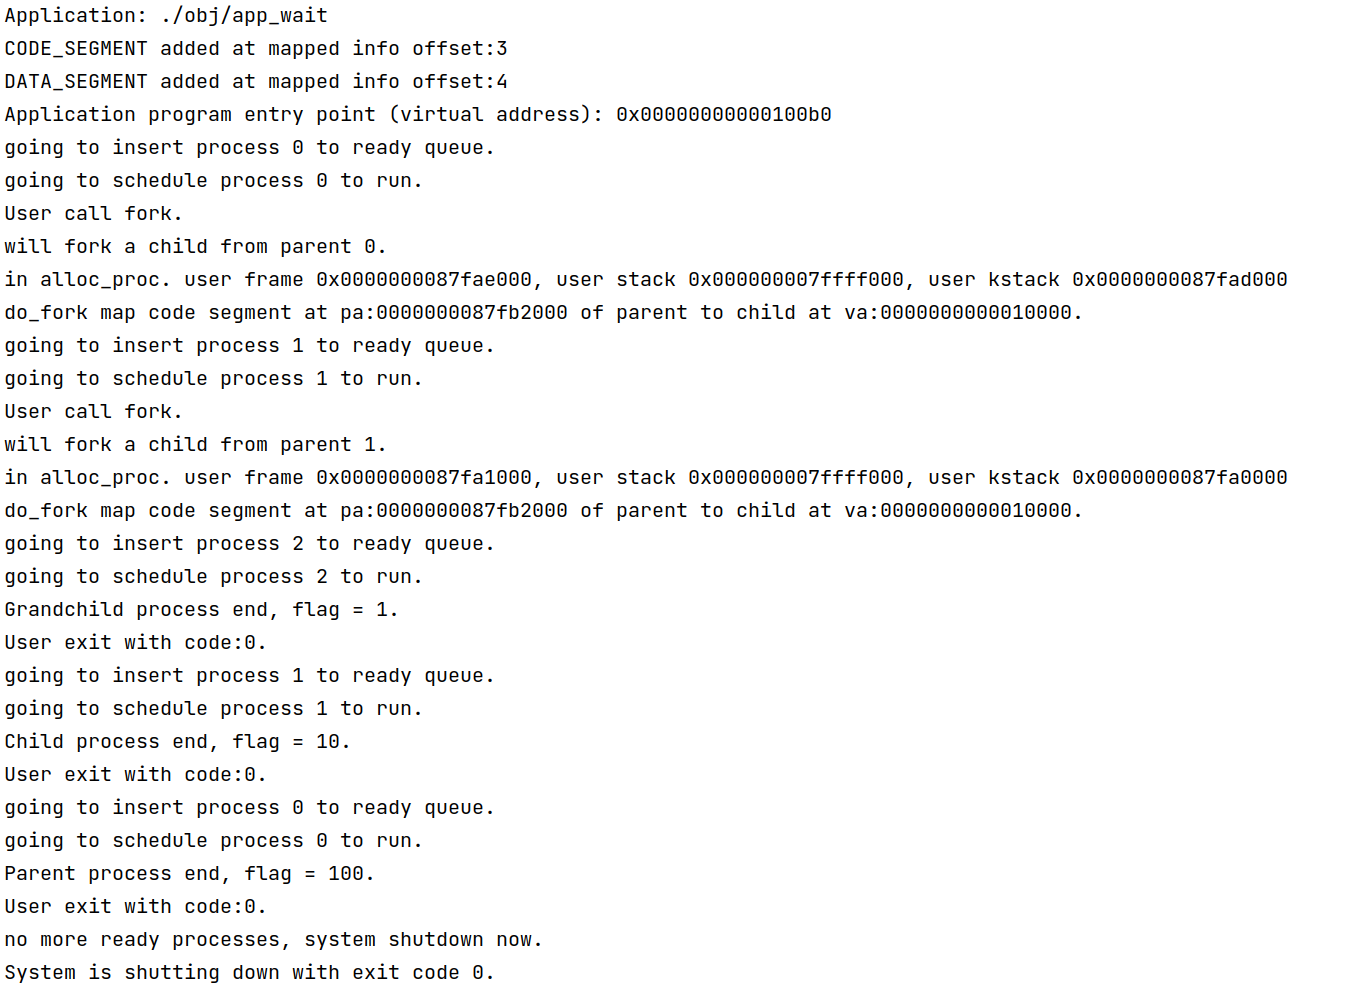
\includegraphics[width = 14cm]{figure/lab3_c1_testresult.png}
    \caption{lab3_challenge1进程等待和数据段复制测试结果}
    \label{fig:lab3-c1}
\end{figure}

\paragraph{lab3_challenge2 实现信号量}
实现信号量实验的测试程序如下。该程序首先创建了一个初值为1的信号量main_sem和两个初值为0的信号量child_sem[2],之后由父进程fork生成子进程,子进程fork生成孙子进程,三个进程分别执行循环次数为5的循环体,并使用信号量的P、V操作轮流打印进程当前的循环次数。
\begin{cppcode}
#include "user/user_lib.h"
#include "util/types.h"

int main(void) {
    int main_sem, child_sem[2];
    main_sem = sem_new(1); 
    for (int i = 0; i < 2; i++) child_sem[i] = sem_new(0);
    int pid = fork();
    if (pid == 0) {
        pid = fork();
        for (int i = 0; i < 5; i++) {
            sem_P(child_sem[pid == 0]);
            printu("Child%d print %d\n", pid == 0, i);
            if (pid != 0) sem_V(child_sem[1]); else sem_V(main_sem);
        }
    } else {
        for (int i = 0; i < 5; i++) {
            sem_P(main_sem);
            printu("Parent print %d\n", i);
            sem_V(child_sem[0]);
        }
    }
    exit(0);
    return 0;
}
\end{cppcode}

编译运行测试程序,程序测试结果如图\ref{fig:lab3-c2}所示。进程0执行fork生成进程1,进程1执行fork生成进程2。进程0首先执行打印,然后释放进程1的资源,并请求进程0的资源;进程1获得进程0释放的资源执行打印,然后释放进程2的资源,并请求进程1的资源;进程2获得进程1释放的资源执行打印,然后释放进程0的资源,并请求进程2的资源,如此循环打印,直至三个进程均打印完毕为止。程序运行结果符合预期,实现信号量的挑战实验成功完成。
\begin{figure}[H]
  \centering
  \subfigure{
    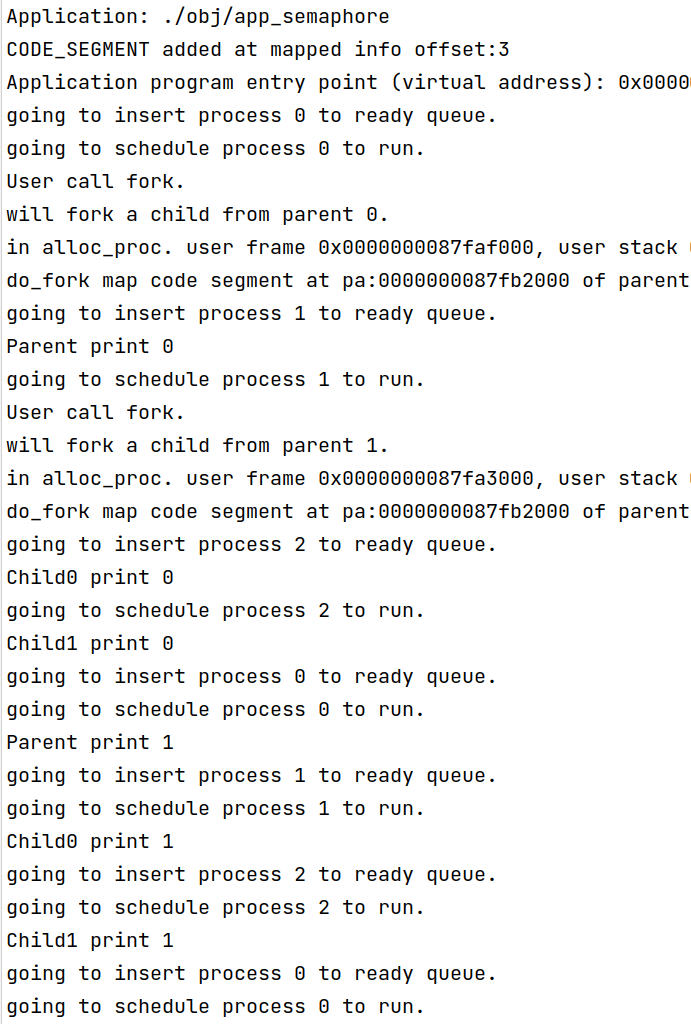
\includegraphics[scale=0.49]{figure/lab3_c2_testresult1l.png}}
  \hspace{0.5in} % 两图片之间的距离
  \subfigure{
    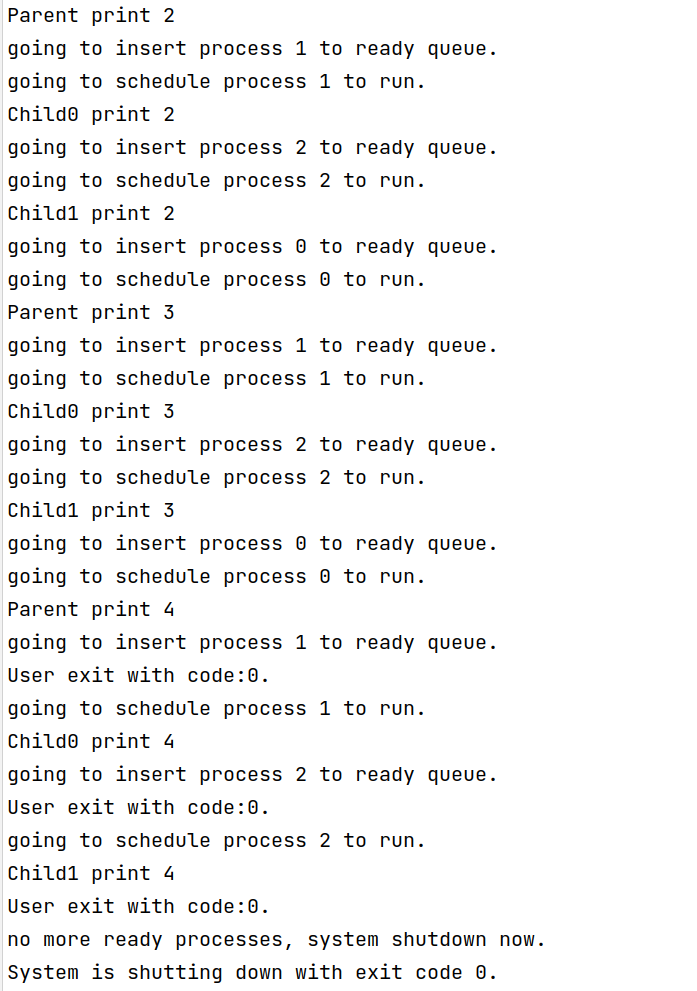
\includegraphics[scale=0.5]{figure/lab3_c2_testresult2l.png}}
  \caption{lab3_challenge2实现信号量测试结果}
  \label{fig:lab3-c2} 
\end{figure}


\subsection{实验心得}
在此次实验中,我对操作系统进程管理相关知识开展了进一步的学习与实践。

首先,我了解并掌握了进程创建的实现原理,通过对进程创建系统调用函数的阅读,以及对代码段映射部分实现的补全,我理解了创建一个进程的实质。

其次,我了解并掌握了操作系统中yield系统调用和进程循环轮转调度这两种方法。yield方法让进程主动释放CPU资源,转进程调度,进而操作系统可以执行其他进程;进程循环轮转调度则是以时间片为单位进行“强制性”的进程调度。

最后,我理解并掌握了进程等待机制,并进一步实现了信号量。一般性的进程等待的实现需要增加一个的进程的等待队列,信号量的实现则可以为每一个信号量设置一个等待队列。进程的等待和信号量都可以作为操作系统中进程同步的实现方法,信号量这一方法的精妙原理至今令我叹为观止。

在此次课程设计中,我完成了9个基础实验和3个挑战实验。在实验过程的初期,我以阅读源码、理解原理为主;在实验过程的后期,尤其是挑战实验的完成阶段,我把注意力更多地放在如何更好地实现我想要实现的功能上。课程设计的完成让我对许多操作系统原理的设计方法有了实践层面上的认知,从许多细小而重要的功能出发窥视了操作系统这样一个庞大体系的全貌。课设给我带来了丰硕的收获,但这只是操作系统原理的基础内容,还有更多现代操作系统的设计技巧与实现方法等待我去慢慢探究。
